%; whizzy chapter -dvi
% -initex iniptex -latex platex -format platex -bibtex jbibtex -fmt fmt
% 以上 whizzytex を使用する場合の設定。
 
%     Tokyo Debian Meeting resources
%     Copyright (C) 2012 Junichi Uekawa
%     Copyright (C) 2011 Nobuhiro Iwamatsu

%     This program is free software; you can redistribute it and/or modify
%     it under the terms of the GNU General Public License as published by
%     the Free Software Foundation; either version 2 of the License, or
%     (at your option) any later version.

%     This program is distributed in the hope that it will be useful,
%     but WITHOUT ANY WARRANTY; without even the implied warranty of
%     MERCHANTABILITY or FITNESS FOR A PARTICULAR PURPOSE.  See the
%     GNU General Public License for more details.

%     You should have received a copy of the GNU General Public License
%     along with this program; if not, write to the Free Software
%     Foundation, Inc., 51 Franklin St, Fifth Floor, Boston, MA  02110-1301 USA

%  preview (shell-command (concat "evince " (replace-regexp-in-string "tex$" "pdf"(buffer-file-name)) "&"))

%%ここからヘッダ開始。

\documentclass[mingoth,a4paper]{jsarticle}
\usepackage{monthlyreport}
% 日付を定義する、毎月変わります。
\newcommand{\debmtgyear}{2014}
\newcommand{\debmtgmonth}{09}
\newcommand{\debmtgdate}{27}
% started from zero:
% (let ((year 2013) (month 7)) (+ (* (- year 2005) 12) month -1))
\newcommand{\debmtgnumber}{117}

\begin{document}

\begin{titlepage}
\thispagestyle{empty}
% タイトルページ:編集必要な部分は最初のマクロに飛ばすこと

\vspace*{-2cm}
第\debmtgnumber{}回 東京エリア Debian 勉強会資料\\
\hspace*{-2cm}

\includegraphics{image2012-natsu/dotdeb.pdf}\\
\hfill{}\debmtgyear{}年\debmtgmonth{}月\debmtgdate{}日

% ここはアップデートすること
% 全角文字にしないとフォントのサイズが合わないので注意
\rotatebox{10}{\fontsize{30}{30} {\gt 特集:DebConf14のビデオ紹介}}\\

\vspace*{-2cm}
\hfill{}
\includegraphics[height=6cm]{image200502/openlogo-nd.eps}
\end{titlepage}

\newpage

\begin{minipage}[b]{0.2\hsize}
 \definecolor{titleback}{gray}{0.9}
 \colorbox{titleback}{\rotatebox{90}{\fontsize{80}{80} {\gt デビアン勉強会} }}
\end{minipage}
\begin{minipage}[b]{0.8\hsize}
\hrule
\vspace{2mm}
\hrule
\begin{multicols}{2}
\tableofcontents
\end{multicols}
\vspace{2mm}
\hrule
\end{minipage}

\dancersection{事前課題}{野島 貴英}

今回の事前課題は以下です:
\begin{enumerate}
 \item 本日、何の作業をやるかを宣言ください。
\end{enumerate}
この課題に対して提出いただいた内容は以下です。
\begin{multicols}{2}
{\small
\begin{prework}{ 野島 }
 xmrisのパッケージ化作業を続ける。
\end{prework}

\begin{prework}{ roger\@localet.com }
お世話になります。Roger です。
初めてなので、特に課題がなし、見学だけをさせていただきます。
宜しくお願い致します。
\end{prework}

\begin{prework}{ dictoss(杉本 典充) }

\begin{itemize}
\item ITP中のwx3.0-docパッケージの修正、パッケージメンテナチームへメールを送る
\item Debian 新メンテナーガイドを読んで理解する
\end{itemize}

\end{prework}

\begin{prework}{ 吉野(yy\_{}y\_{}ja\_{}jp) }

DDTSS\footnote{\url{http://ddtp.debian.net/ddtss/index.cgi/ja}}

\end{prework}

\begin{prework}{ henrich }

\begin{itemize}
\item net-snmpパッケージのバグレポートを眺める
\item debianjpでの改善案を練る
\end{itemize}

\end{prework}

\begin{prework}{ 野首(\@knok) }
\begin{itemize}
\item groongaのドキュメント整備
\item jessieインストーラの調査
\item libsixelのパッケージ化 \\
\url{https://github.com/saitoha/libsixel}
\end{itemize}
\end{prework}


}
\end{multicols}

\dancersection{Debian Trivia Quiz}{野島 貴英}

 Debianの昨今の話題についてのQuizです。

今回の出題範囲は\url{debian-devel-announce@lists.debian.org} や \url{debian-news@lists.debian.org}に投稿された
内容などからです。

\begin{multicols}{2}
%; whizzy-master ../debianmeetingresume201311.tex
% 以上の設定をしているため、このファイルで M-x whizzytex すると、whizzytexが利用できます。
%

\santaku
{FSFがDebian Projectへ案内をしてきた、自由ソフトウェアのみの元で動かすことの出来るハードウェアについてのデータベースは次のうちどれ?}
{h-node.org}
{wiki.debian.org/Hardware}
{openbenchmarking.org}
{A}
{日本語の本件のニュースはsourceforge.jpの記事参照:http://sourceforge.jp/magazine/14/09/11/062900 。FSFはmainリポジトリのみのパッケージで構成されるDebianは自由ソフトウェアとみているとのこと。}

\santaku
{Debconf14の参加人数は結局何人?}
{900人}
{300人}
{1000人}
{B}
{300人とのことです。参考:Debconf13は290人、Debconf12は176人、Debconf11は335人でした。}

\santaku
{8/17にbuilddにて使われるアーカイブがどこからもアクセスできるようになりました。urlはどれ?}
{ftp.debian.or.jp/debian/}
{ftp.jp.debian.org/debian/}
{incoming.debian.org/debian-buildd/}
{C}
{今までは、どこからもアクセスできたわけではなかったようです。}

\santaku
{2014/8/19に登録商標としてDebianロゴが正式に登録されたそうです。どこの国の登録商標でしょうか?}
{米国}
{日本}
{スイス}
{A}
{United States Patent and Trademark Officeになります(つまり米国。)登録されたDebianロゴのデザインは http://tdr.uspto.gov/search.action?sn=86037470 からたどると閲覧できます。}

\santaku
{2014/8/24のBitFromDPLによれば、Debian Projectは仮想通貨による寄付をはじめて受け付けたそうです。具体的には何という仮想通貨でしょう?}
{Greeコイン}
{Crysta}
{BitCoin}
{C}
{Debian ProjectはBitCoinをそのまま受け付けることが出来るシステムを持たないため、その場限りの方法で受け取ったとのことです。今後、こういった仮想通貨での寄付の受け取りと取り扱いについて意見がほしいとのことです。}

\santaku
{検索エンジンのDuckDuckGOより、収入が入ったとのことです。2014/8/24現在、月当たりのDuckDuckGOからの平均収入は月額いくらでしょう?}
{\$10}
{\$152}
{\$1400}
{B}
{Debianパッケージに含まれるブラウザにデフォルトで登録されている検索エンジンの候補としてDuckDuckGOが搭載されていることによる収入となります。DuckDuckGOはプライバシーに配慮した検索エンジンです。最近は、iphone のsafariブラウザにあらかじめ登録される検索エンジンの候補としても上がり有名になりつつあります。URLはhttps://duckduckgo.com/}

\santaku
{2014/8/27にDebian archiveに搭載された2つの新しいアーキテクチャは、arm64以外には以下のどれ?}
{sparc}
{mips}
{ppc64el}
{C}
{ 64 bit powerpcのlittle endianモードのポーティングとのことです。すでに存在するppc64はbig endianのバイナリのポートティングとなります。}

\santaku
{2014/8/31にて、arm64ポートのDebian開発用に、無償のARM64用のコンパイラ・デバッガ等の開発キットの提供が行われたようです。製品名は以下のどれ?}
{Microsoft Visual Studio}
{IAR Embedded Workbench}
{DS-5 Development Studio}
{C}
{ Debian Editionとのことです。アナウンスによれば、ダウンロードリンクは http://ds.arm.com/debian/ からダウンロード可能とのことですが、日本からはダウンロードが現在出来ない模様です。残念!もちろんですが、この開発キットは無償ではあるものの自由ソフトウェアではないので誤解なきよう。}

\santaku
{ Debian keyringからある大きさ以上の秘密鍵長を持たないキーが2014/12/31以降で削除される事についてのリマインドのアナウンスが流れていました。ある大きさとは以下のどれ?}
{ 512bit }
{ 2048bit }
{ 4096bit }
{B}
{ キーサインにつかうgpgの鍵も2048bit以上にしましょう!}

\santaku
{ 2014/9/17にDebian Policy が改定されました。改定後のバージョンはいくつ?}
{ 3.9.5.0 }
{ 3.9.6.0 }
{ 4.0.0.0 }
{B}
{ パッケージ開発をする前に、新しいDebian Policyの変更差分は読んでおきましょう。}

\end{multicols}

\dancersection{最近のDebian関連のミーティング報告}{野島 貴英}

\subsection{第116回東京エリアDebian勉強会}

 東京エリアDebian勉強会116回目は(株)スクウェア・エニックスさんで開催されました。
 
 9人の参加者がありました。セミナは、なかおさんにて、Debianでタイルマップサーバーを作り、
JAXAで公開されている海水表面温度データをOpenStreetMapに重ねて表示する件についての
発表が行われました。

 地球観測衛星から送られてくる地球の海水表面温度がDebianにより処理されて図示される様は圧巻でした。
データそのものは地球規模のサイズを対象している為、非常に膨大な量のデータを扱うことになり、
そのままではズーム処理にて処理が非効率になってしまうところを、部分的に処理するやり方に
変更してうまく処理されていました。なお、本しくみを使ったサービスは
ISAC Tokyo 2014(\url{http://tokyo.spaceappschallenge.org/2014_tokyo.html})
にて発表されており、賞も受賞したとのことです。地球規模や、ISACといった、非常にスケールの大きい事を対象にするお話を聞くことができ、非常に新鮮でした。

 また、飛び込みではありますが、zinraiさんによる構成管理ツールのAnsibleについてのBOFが行われました。DebianでのAnsibleの現状と実際の使い方の例について、ディスカッションをしました。

 発表の後はもくもく会を行い、最後に各自で成果発表を行いました。

 宴会は「路島と喰らえ 新宿東口靖国通り店」で行いました。

% % (query-replace-regexp "<.*?>" "")
% % (query-replace-regexp "^[	 ]\+" "")

%-------------------------------------------------------------------------------
\dancersection{DebConf14のビデオ紹介}{野島 貴英}
%-------------------------------------------------------------------------------
\index{debconf14-video-intro}

\subsection{DebConf14}

 DebConfとは毎年1回Debian Project主催で開かれる大きなカンファレンスのことです。

 そこでは、世界中からDebian Projectの活動に興味を持つ方々が集まり、Debianの開発や貢献についての
発表や活発な議論が行われています。

 今年は第15回目のカンファレンスとなり\footnote{DebConf0が存在するので、全部で15回目です。}、8/23〜8/31の間、米国オレゴン州ポートランドにて、DebConf14と
して開かれました。

 ここでは、DebConf videoチームにより公開されているDebConf14のカンファレンスの各セッションのビデオ
を視聴し語ってみます。

\subsection{DebConf14のビデオに関する情報}

 DebConf14のスケジュールと、開かれたセミナの概要などの情報は、DebConf14の公式ホームページの\url{http://debconf14.debconf.org/}を見て下さい。

 セミナとBOFの動画ファイルは、\url{http://meetings-archive.debian.net/pub/debian-meetings/2014/debconf14/webm/}にwebmフォーマットでおいてあります。video codecはvp8、audio codecはvorbisという、Debianらしくオープンな技術に拘ったデータ形式となっているのが特徴です。

\subsection{視聴するにあたって補足}

 大量のビデオが公開されており、また時間も1時間弱程度はあるので、きっと本勉強会にいらっしゃるような熱心なDebian関係者の方は、
そのままのスピードで視聴するのではなく、早回しで視聴したいという要望を持たれる方がいらっしゃると思います。そんな時には、
mplayer2をお勧めしておきます。

\begin{commandline}
$ apt-get install mplayer2
$ mplayer2 <動画ファイル名>
\end{commandline} 

 また、起動するとわかるのですが、あまり親切なメニューは出てきません。代わりにman mplayerするとわかるのですが、
豊富なショートカットキーがあり、こちらを使う事により再生を制御できます。(表\ref{tab:mplayer-key}参照)


\begin{table}[ht]
\begin{center}
\begin{tabular}{|l|p{7cm}|l|p{7cm}|}
\hline 
キー&操作 &キー & 操作\\ \hline \hline
[ & 10\%スロー & ] & 10\%スピードアップ \\ \hline 
$\leftarrow$ & 1分戻し & $\rightarrow$ & 1分スキップ \\ \hline
$\uparrow$ & 10分戻し & $\downarrow$ & 10分スキップ \\ \hline
o & 残り時間/再生時間表示(複数回押す) & q & mplayerを終了\\ \hline
\end{tabular}
\end{center}
\caption{mplayerのショートカットキー}
\label{tab:mplayer-key}
\end{table}

 また、英語の聞き取りが苦手な方には、DebConf subtitle projectらによる、英語による書き起こしのテキストデータが入手できます。
gitからの入手の仕方は以下のとおりです。

\begin{commandline}
apt-get install git
git clone http://anonscm.debian.org/git/debconfsubs/debconfsubs.git
cd debconfsubs/2014/debconf14/english/wip/
\end{commandline}
 
 2014/9/25現在のところ、未完成のものも含めて9つのセッションに関する書き起こしデータが手に入るようです。
なお、.srtの拡張子を持つデータは字幕データであり、字幕ファイルを扱える動画プレイヤーで字幕を表示しながら
セッションの動画を視聴することが出来ます。こちらについての操作方法の例は、第105回東京エリアDebian勉強会のセミナ
資料\cite{ref:osc-tokyo-2013-fall}に具体的に記載していますので、こちらを参考にしてください。

 さらに、gitに格納されるよりも早く字幕の英文を見たい、あるいは、そもそも自分で英文字幕を起こす手伝いをしたい人は、
\url{https://wiki.debconf.org/wiki/Videoteam/Subtitles}で紹介されている\url{http://www.amara.org/}
の字幕書き起こし用のWEBサービスにアクセスしてください。こちらのページから起こし途中の字幕を閲覧したり、
字幕付きのDebConf14のセッションの動画を実際に見ることが出来ます。

\subsection{DebConf14大物ゲスト}

 今回は、Debianに直接の関係はあまりないのですが、大物ゲストが呼ばれており、専門のセッションが開かれています。

 \subsubsection{Q\&A with Linus Torvalds}

\begin{wrapfigure}{r}{5cm}
  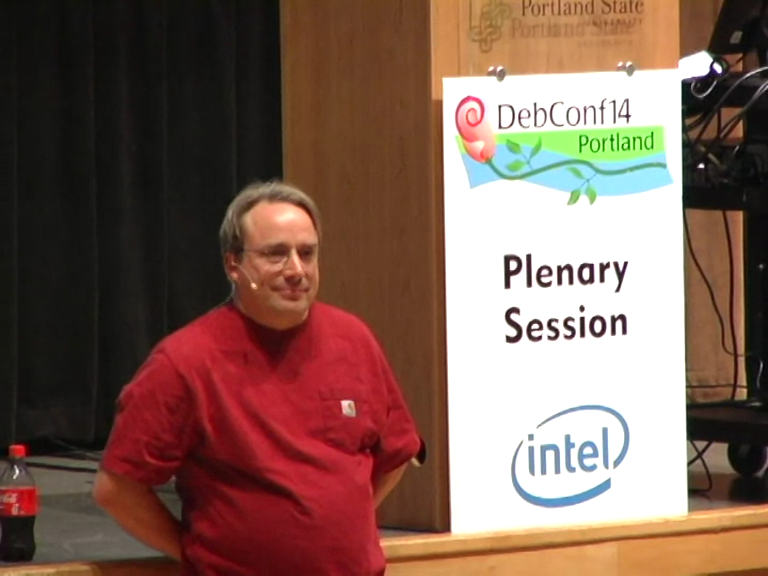
\includegraphics[width=5cm]{image201409/qa_linus.png}
\end{wrapfigure}

  Linuxカーネルの最初の作者であるLinus Toravalds本人を呼んで、セミナ参加者から一人づつ質問を受け続けるというセッションです。

 \begin{itemize} 
  \item Linusさんの関心のほとんどはLinuxカーネルそのものに費やされており、ディストリビューションの動向についてはあまり気にしてないようです。
Debianも1度試したきりで結局Macに入れようとして失敗しただけのようで(Ubuntuも同様)。
  \item gccの件や、systemdの件など、次々と一見答えにくい(?)質問が次から次へとLinusさんにぶつけられていました。特にsystemdの件ではLinusさんもコミュニティでの扱いについて熱い答弁をされていました。
  \item GPUとkernelの関係などについて昨今の事情についての質問もありました。
  \end{itemize}

 最初の質疑でLinusさんも非常に気楽に答えていたためうっかり、品位に欠ける表現がところどころ飛び出してしまい、女性のDebConfスタッフ(Debian Womenの方)に表現の注意を受ける一幕もありました。

 \subsubsection{Weapons of the Geek} 

\begin{wrapfigure}{r}{5cm}
  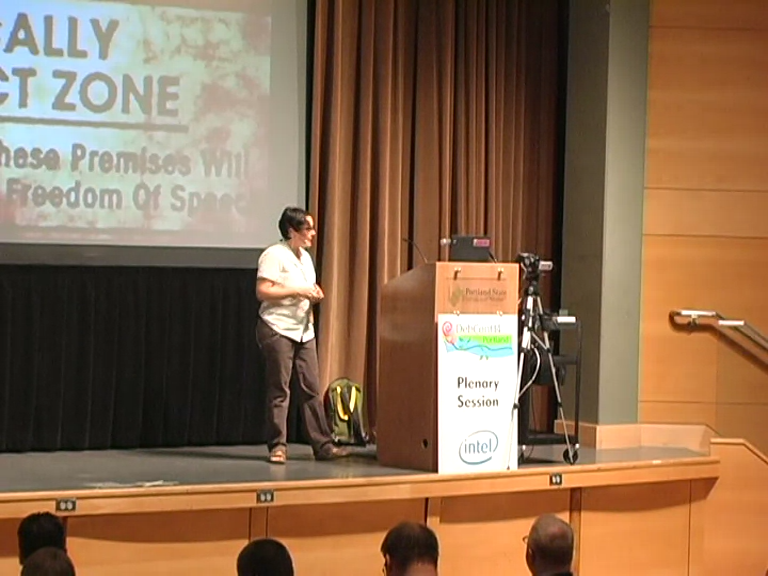
\includegraphics[width=5cm]{image201409/weapon_geek.png}
\end{wrapfigure}

 クラッカー集団であるAnonymousについての社会面、文化面の研究で有名な、Gabriella Colemanさんのセッション。AnonymousとAnonymousを取り巻く独特のハッカー文化の解説と考察を行うというセッション。日本にはほとんど馴染のないサブカルチャー(例:XENU,Chanology,Scientologyなど)の紹介と、これらに対するAnonymousの考え方への影響などの紹介があって面白いです。

\subsection{Debianの主なトピック}

\subsubsection{Bit From the DPL}

\begin{wrapfigure}{r}{5cm}
  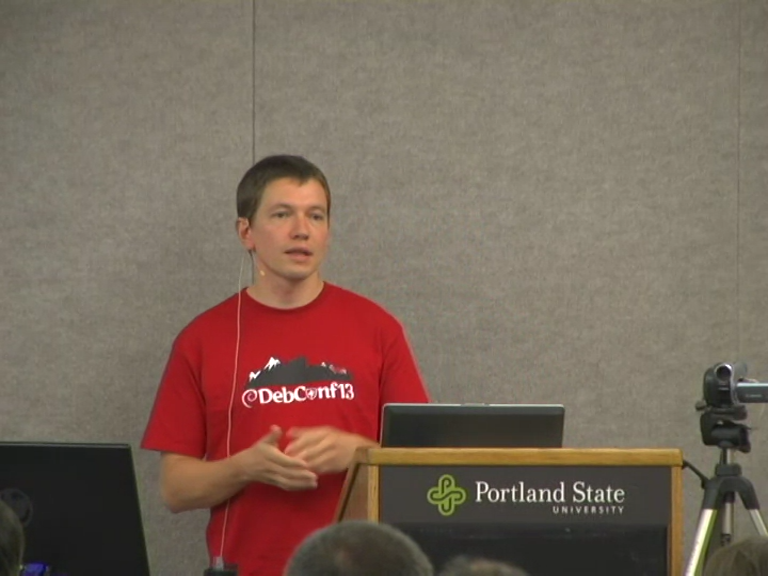
\includegraphics[width=5cm]{image201409/bit_dpl.png}
\end{wrapfigure}

 2014年もDPL続投のLucas Nussbaumさんのプレゼン。

 プレゼン資料は、\url{http://blop.info/p/201408-dc14-dpl.pdf}で公開中。

 \begin{itemize}
 \item Debian Projectの収支の件の話が出ました。Debian Projectは資産をTrusted Organizationとして認めた機関にあずけているのですが、全部あわせると、日本円で約2,800万円ぐらいある模様です。保有割合としては、SPI(米国/US\$預かり)が最も多い状況です。さらに、DebConfの度にスポンサーからの寄付を使い切れず資産が増えてしまう模様で、ここ2年がその傾向が顕著とのことです。
 \item さらなる予算の活用についてのディスカッションが行われました。予算利用の候補としての案は以下の4つ。
   \begin{enumerate}
      \item Debianの普及に使う(例:mini-DebConfをもっと開く。景品(Tシャツなど)を新しい貢献者へ配る、Debianのブースの何かに使う)
      \item セキュリティに関して強化。Debian公式開発者へ暗号化用スマートカードを配る。
      \item 開発の効率化に活用(例:Sprintの活発な開催、開発用ハードウェアを充実させる、DebConfへのtravelスポンサーの増資)
      \item upstreamとの積極的なコミュニケーションの為に活用(例:upstreamについてのカンファレンスへの参加の旅費。upstreamの接待など)
   \end{enumerate}
   会場では参加者の挙手を募り、賛否の割合を確認していました。
 \end{itemize}

 \begin{itemize}
 \item Debian Projectに関してSWOT解析をされていました。SWOTのうち、弱み(Weaknesss)としては、中核部分に関しての完全な人手不足、技術的でない部分への興味のなさと協力者の不足、Debian開発者同士でノウハウの共有化が行われていない場合がある、パッケージ化が難しい、メンター不足やそもそも必要な技術力が高いなどで新参者の開発参加のハードルが非常に高い、upstreamとのコミュニケーションが薄いという点が挙げられていました。脅威(Threats)としては、他のディストリビューションではすでに解決済みのことに対応できていない、Debianの活動をするのに必要なスキル(開発とシステム管理作業など)を習得するような大学のカリキュラムがない、他プログラミング言語が独自で持つパッケージシステムとDebianパッケージの比較をされてしまうが挙げられていました。
\end{itemize}

\subsubsection{Jessie bits from the release team}

\begin{wrapfigure}{r}{5cm}
  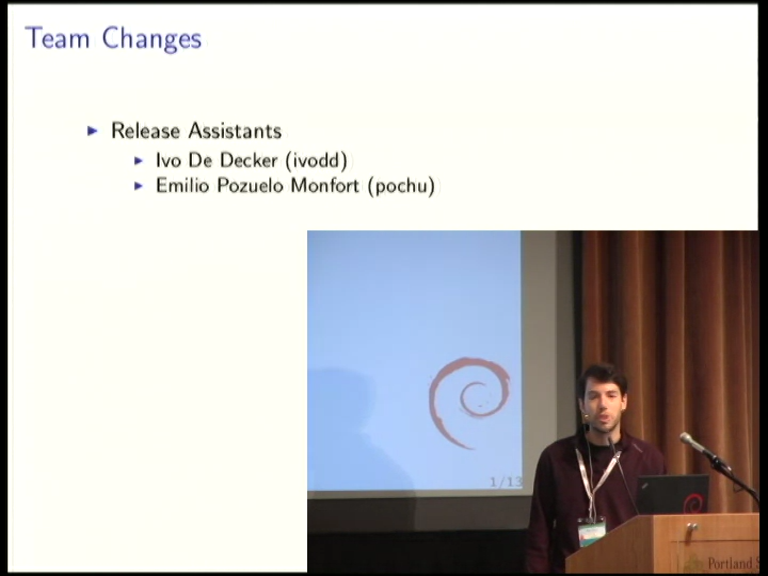
\includegraphics[width=5cm]{image201409/jessie_release.png}
\end{wrapfigure}

 Releaseチームのセッションです。

 スライドは\url{https://release.debian.org/talks/debconf14/rt-debconf14.pdf}

 主な内容として、

\begin{itemize}
  \item freezeまでのタイムスケジュールと内容は以下の通り。
    \begin{itemize}
    \item 9/5に新規のtransitionを止める(ライブラリのアップグレードはここで終了)
    \item 10/5より緊急のアップロードを無視しはじめ、testingへの移行に10日かかるようになる。また、セキュリティチームからサポート不可のパッケージの吟味が行われるようになる。
    \item 11/5 Freezeする。
    \end{itemize}
\end{itemize}

\begin{itemize}
  \item 現在のRC bugの残りは450個。2/5以降、testingに移動するのが望ましくないと判断されたパッケージはremoveされる。基本的にどのパッケージもremoveから無事だとは思わないでほしいとのこと。
  \item 今から注意してほしい点として、今からはもう新規のtransitionを提案しないでほしい、Jessieに入れる気の無いパッケージのアップロードは一旦やめてほしい、とにかくインストールテスト(特にUEFI対応のPCを持っている人はできるだけ協力タノムとの事)と、バグを潰してほしいとのことです。
\end{itemize}

\subsection{日本の参加者の方の発表}

 今回、2名の日本からの参加者の方が発表をされていましたのでここに紹介しておきます。

\subsubsection{My PGPGPG key is RSA 2048bit but I put the private key on Gnuk Token}

\begin{wrapfigure}{r}{5cm}
  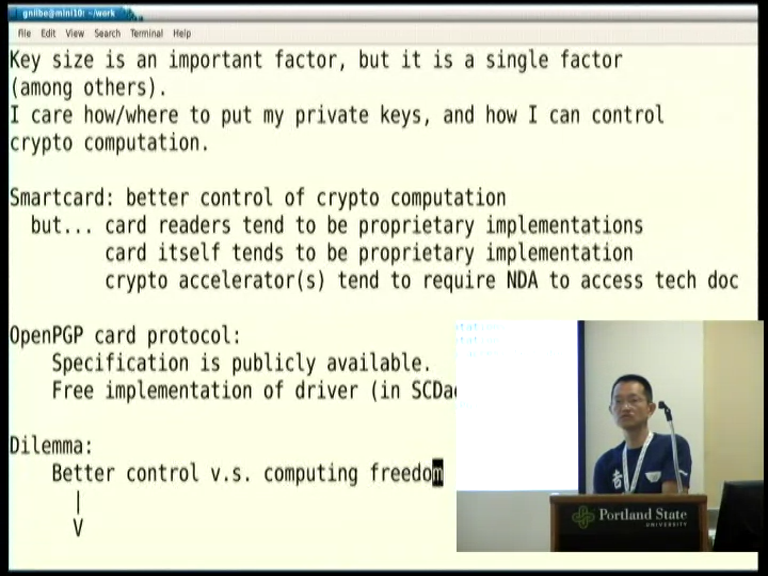
\includegraphics[width=5cm]{image201409/gnuk.png}
\end{wrapfigure}

 新部さんのセッション。

 内容はGnuk Tokenの歴史と構造、動作の仕組みについてのセッションです。動作デモもありました。

 スライドは、\url{http://gobby.debian.org/export/debconf14/bof/gnuk}

 \begin{itemize}
  \item Gnuk Tokenは、gpgのセキュリティスマートデバイスとして動作できるUSBドングルの事。新部さん開発。このドングルを利用してgpgサインを行えば、暗号処理もドングル内部で行うため秘密鍵を不正に取り出されることもなくセキュアに署名・暗号化が出来る。    
 \end{itemize}

 \begin{itemize}
  \item Gnuk Tokenでは、乱数発生機として、未接続の内蔵ADコンバータの1ビット目を使ったとのこと。
  \item Gnuk Tokenは最大3つの鍵を扱えるとのこと。ストア可能なキーサイズは2kbytesはストアできる。
 \item 動作速度として、1.5秒でDebianパッケージのgpgサインが可能。
  \end{itemize}

 途中、ドングル売ってくれとの聴講者の要望があったのが印象的でした。

\subsubsection{find \& imporove some bottleneck in Debian project}

\begin{wrapfigure}{r}{5cm}
  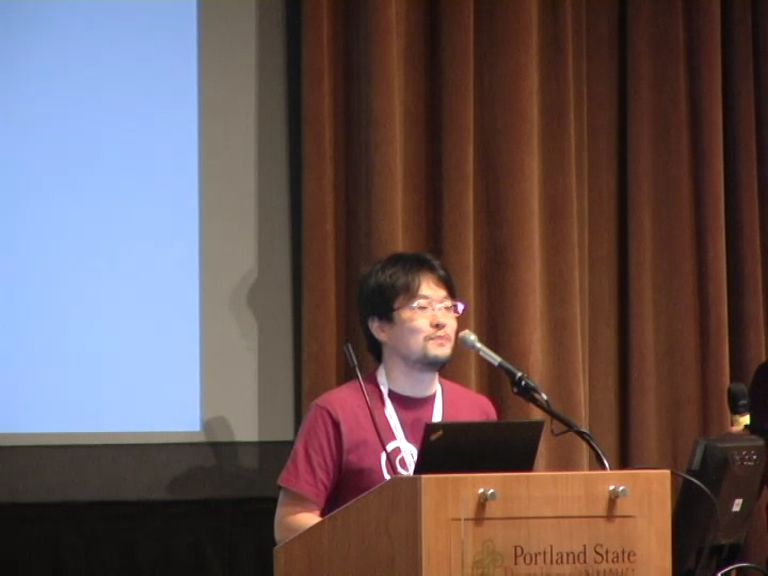
\includegraphics[width=5cm]{image201409/find_improve.png}
\end{wrapfigure}

 やまねさんによるライトニングトーク(以下LT)中の発表。動画ファイル名Lightning\_Talks\_4.webm中 0:43:14あたりで発表。

 スライドは\url{http://www.slideshare.net/henrich_d/find-improve-some-bottleneck-in-debian-project-debconf14-lt}

 \begin{itemize}
  \item NEW キューのftpmasterによるチェックに時間がかかる事を解決したいという内容。現在ftpmasterだけが膨大な量のパッケージのレビュー作業・差し戻し作業をやっている事により、作業量が多すぎてNEW キューの受け入れが滞りがちという問題がある。
  \item ここでreview contributorという人を募集し、ftpmasterが現在行っているNEW キューのパッケージチェック作業を、彼ら(複数人)にやらせ、ftpmasterは最終の受け入れのOK/NGのみ出す役割にする。
 \end{itemize}

 \begin{itemize}
 \item review contributorは、Debian開発者候補としての訓練にも良いし、ftpmasterの作業が過多になってNEW キューが滞るのも解決できて一石二鳥でウマーというのがメリットなので、どうでしょう?という提案。
\end{itemize}

 こちらをきっかけに、Debian Projectに採用されると良いと思いました。

\subsection{その他}

 その他発表で興味深い内容のものを紹介します。

 \subsubsection{Debian in the Dark Ages of Free Software}

\begin{wrapfigure}{r}{5cm}
  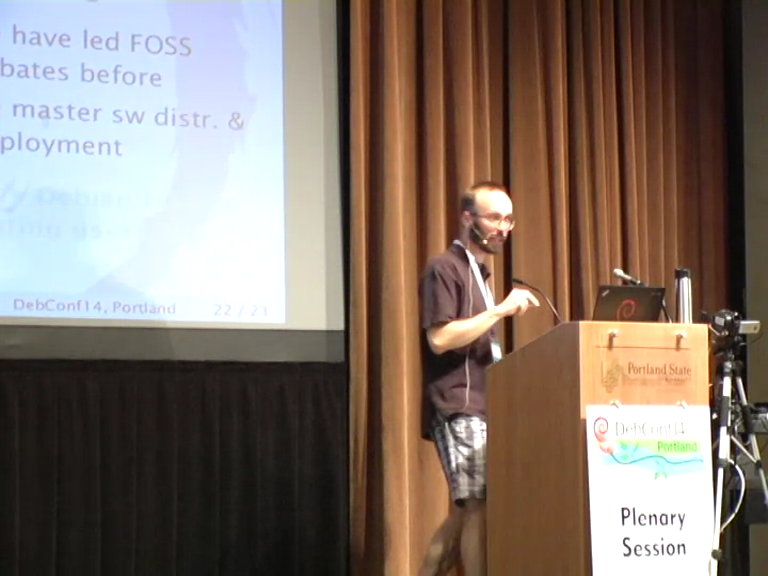
\includegraphics[width=5cm]{image201409/dark_age.png}
\end{wrapfigure}

 2012年のDPLであったStefano Zacchiroli(以下zack)さんの発表です。

 \begin{itemize}
  \item DebianはDFSG Freeなdistoributionを作り普及させたことでは一定の成功を収めた。
 \item OSSも大変身近なものになり、ユーザは、たくさんのソフトウェアについて改変の自由が提供されるようになった。
  \item しかしながら、これらが成功した一方で、クラウドサービスも進化したため、せっかく勝ち取ったはずのソフトウェアの自由が、クラウドサービスの普及により、結局ユーザの手から取り上げられつつある。
 \item また、自由(Free)Softwareを作るにはFreeの開発ツール/開発環境が究極的には必須であるにもかかわらず、github/Gmailなどユーザからみれば自由でないサービスが益々開発ツール/環境としての地位を強固なものにしている。
 \end{itemize}

 \begin{itemize}
 \item このような時代にある事を認識し、これを自由(Free) Softwareの暗黒時代と呼ぼう。
\end{itemize}

 セッションでは、zackによるアイデアも披露され、また聴講者からも提案があったものの、zack曰くはっきりとした良い解決方法はまだ自分にもわからないという事でした。
 
 このセッションで示されている問題は、難しく由々しき問題です。共感される方は是非議論に提案に加わっていただけると幸いです。

\subsection{おわりに}

 他にもいろいろなセッションの動画が公開されています。ここでは紹介しきれなかったセッションにも面白いものが多数あります。

 興味がある方は是非視聴くださいませ。また、英語のヒアリングに自信のある方はDebConf Video subtitleチームに作業のご協力をおねがいします。

\begin{thebibliography}{9}
\bibitem{ref:osc-tokyo-2013-fall}OSC 2013 Tokyo/Fall 東京エリアDebian勉強会セミナ資料, \url{http://tokyodebian.alioth.debian.org/pdf/ debianmeetingresume201310-presentation.pdf}
\end{thebibliography}

%-------------------------------------------------------------------------------
\dancersection{会場での無線LANのつなぎ方}{野島 貴英,Roger}
%-------------------------------------------------------------------------------
 \subsection{はじめに}

 今回試験として、会場側でフィルタ無しのグローバル回線を用意しました。
ただ、会場側のセキュリティポリシーにより、wpa-psk AES hidden SSIDという
方式での提供となります。

 以下にDebianマシンでの接続方法を記載します。

 また、自分の環境では違うやり方でつながったという方は、野島まで
教えて下さい。こちらでもノウハウとして溜めていく予定です。

 \subsection{wpasupplicant及び/etc/network/interfacesを利用の場合}

 もっとも良いマニュアルは、/usr/share/doc/wpasupplicant/README.Debian.gz
となります。困った場合はこちらも合わせてご参照下さい。

 以下に/etc/network/interfacesの定義について会場の例を記載します。

\begin{commandline}
$ sudo vi /etc/network/interfaces
-----以下のエントリがなければ追記ここから----------
iface wlan0_debian inet dhcp
     wpa-conf /etc/wpa_supplicant/wpa_supplicant_debian.conf
-----以下のエントリがなければ追記ここまで----------
$ sudo vi /etc/wpa_supplicant/wpa_supplicant_debian.conf
-----以下のエントリを追記ここから----------
network={
     ssid=<<会場のSSID>>
     psk=<<会場のパスワード>>
     scan_ssid=1
}
-----以下のエントリを追記ここまで----------
$ sudo chmod 600 /etc/wpa_supplicant/wpa_supplicant_debian.conf
$ sudo ifup wlan0=wlan0_debian
\end{commandline}
%$

 また、ハマってしまった時のデバッグ方法は、
/usr/share/doc/wpasupplicant/README.Debian.gz中の''4. Trubleshooting''の章が便利です。

 \subsection{その他の無線LAN用パッケージを利用の場合}

 すみません、自分が情報を持たないため、現場で教えて下さい。

\newpage
\center{\LARGE メモにお使い下さい}
\newpage
\center{\LARGE メモにお使い下さい}

\cleartooddpage

\vspace*{15cm}
\hrule
\vspace{2mm}

\includegraphics[width=2cm]{image200502/openlogo-nd.eps}
\noindent \Large \bf Debian 勉強会資料\\
\noindent \normalfont \debmtgyear{}年\debmtgmonth{}月\debmtgdate{}日 \hspace{5mm}  初版第1刷発行\\
\noindent \normalfont 東京エリア Debian 勉強会 (編集・印刷・発行)\\
\hrule

\end{document}
